\section{Results}\label{sec:results}

We answer five questions:
\begin{enumerate}
\item How well does SpatialNet find the pointed-at object, compared with published results of state-of-the-art and zero-shot models and with simple references (Section~\ref{sec:main})?
\item Where does it fail, by distance and by head (Section~\ref{sec:heads-results})?
\item Which design choices matter (Section~\ref{sec:ablations})?
\item Does it follow the wearer's hand when other hands are visible (Section~\ref{sec:own})?
\item How fast does it run on the glasses (Section~\ref{sec:ondevice})?
\end{enumerate}
SpatialNet numbers are from one training run (seed 42) on the 3,029 test images. \tbd{After T4, report mean $\pm$ std over three seeds.}

\subsection{Pointed-Target Localisation}\label{sec:main}

\paragraph{References.} We compare SpatialNet with two kinds of reference.
\begin{itemize}
\item \emph{Published results.} We copy these numbers and do not re-run the models.
  \begin{itemize}
  \item VistaRef~\cite{li2026vistaref} and PointVG-R~\cite{li2026pointvgr} report results on the same 3,072-image test split; ours omits 43 unclear images and the 425 images without a target. PointVG-R also reports zero-shot and fine-tuned multimodal LLMs on that split.
  \item EgoPoint-Ground's pointing-only (POG) results~\cite{egopoint} come from a different setting: zero-shot models receive the ground-truth hand box, and the evaluated subset is not stated.
  \end{itemize}
\item \emph{Simple references.} These test whether knowing where the fingertip is would be enough:
  \begin{itemize}
  \item the mean training target box at a fixed position;
  \item a box of mean training size centred on SpatialNet's predicted fingertip;
  \item the same box centred on the ground-truth fingertip.
  \end{itemize}
\end{itemize}

\begin{table}[t]
  \caption{Localisation of the pointed-at target on the EgoPoint test split. All columns compare a predicted \emph{target} box with the labelled target box; hand accuracy is in Table~\ref{tab:heads}. Our rows use the 2,604 test images with a target; the 425 no-hand images have none. mIoU and P@$\tau$ (Section~\ref{sec:metrics}) in \%, the published values multiplied by 100. We count IoU${\geq}\tau$, as does VistaRef; EgoPoint-Ground and PointVG-R count IoU${>}\tau$. \emph{Far}: P@0.5 on the 209 far targets. Latency per image on the hardware named in the text; only SpatialNet runs on the glasses.\\
  $^\ast$\,VistaRef~\cite{li2026vistaref}, Table~1, setting ``Train-Real Data Test'', BEiT-3-L backbone (226M parameters with BEiT-3-Base); test set of 3,072 images, which includes no-hand images.\\
  $^\ddagger$\,PointVG-R~\cite{li2026pointvgr}, Table~1, EgoPoint-CoT test set, built on the same 15,455-image release and 3,072-image test split.\\
  $^\dagger$\,EgoPoint-Ground~\cite{egopoint}, Table~4, pointing-only (POG) task: inference only, given the ground-truth hand box; the evaluated data subset is not stated.\\
  How the published works score images without a target is not stated; our rows exclude them.}
  \label{tab:main}
  \footnotesize
  \setlength{\tabcolsep}{4pt}
  \begin{tabular}{lrrrrrrr}
    \toprule
    Method & Params & P@0.3 & P@0.5 & P@0.7 & mIoU & Far & Latency \\
    \midrule
    \multicolumn{8}{l}{\emph{Published, trained on EgoPoint (not re-run)}} \\
    \quad VistaRef$^\ast$, image + fixed prompt & $>$226M & 97.0 & 93.9 & 82.6 & 82.0 & -- & -- \\
    \quad PointVG-R$^\ddagger$, image + instruction, SFT + RL & 7B & 88.1 & 83.6 & 74.5 & 75.7 & -- & -- \\
    \quad Qwen2.5-VL-7B$^\ddagger$, image + instruction, SFT & 7B & 68.7 & 63.6 & 56.7 & 59.8 & -- & -- \\
    \multicolumn{8}{l}{\emph{Published, zero-shot (not re-run)}} \\
    \quad Qwen2.5-VL-7B$^\ddagger$, image + instruction & 7B & 54.2 & 49.8 & 42.9 & 45.5 & -- & -- \\
    \quad Qwen3-VL-8B$^\ddagger$, image + instruction & 8B & 48.1 & 44.5 & 39.0 & 43.0 & -- & -- \\
    \quad SV-CoT$^\dagger$, image + hand box & $>$1B & 69.4 & 63.9 & 55.6 & -- & -- & -- \\
    \quad Qwen3-VL-4B$^\dagger$, image + hand box & 4B & 67.1 & 61.2 & 53.2 & -- & -- & -- \\
    \multicolumn{8}{l}{\emph{Simple references}} \\
    \quad Mean training box, fixed position & 0 & 41.3 & 9.6 & 0.9 & 27.4 & 4.3 & -- \\
    \quad Mean-size box at predicted fingertip & 0.72M & 43.5 & 11.2 & 0.9 & 28.8 & 0.0 & -- \\
    \quad Mean-size box at true fingertip (oracle) & -- & 43.6 & 11.4 & 1.0 & 29.0 & 0.0 & -- \\
    \midrule
    \textbf{SpatialNet} (image only, seed 42) & 0.72M & 78.6 & 58.9 & 31.8 & 53.3 & 25.4 & \xx\,ms \\
    \quad $\pm$ std over 3 seeds & & \xx & \xx & \xx & \xx & \xx & \\
    \bottomrule
  \end{tabular}
\end{table}

\paragraph{Results.} Table~\ref{tab:main} gives three findings.
\begin{itemize}
\item \emph{The target head does real work.} Knowing the fingertip is not enough: a mean-size box at the true fingertip reaches a P@0.5 of only 11.4\% (12.0\% when shifted by the mean training offset), because target sizes vary widely (2.6\% to 44\% of the image area, 10th to 90th percentile). SpatialNet reaches 58.9\%.
\item \emph{Large models trained on EgoPoint are far more accurate.} SpatialNet is 35 points below VistaRef in P@0.5 and 51 points below in P@0.7, where its boxes are least precise; in mIoU the gap is 29 points (53.3 against 82.0). It is 25 points below PointVG-R, and 4.7 points below Qwen2.5-VL-7B fine-tuned on the same data.
\item \emph{It is comparable to zero-shot multimodal LLMs.}
  \begin{itemize}
  \item SpatialNet's P@0.5 (58.9\%) and mIoU (53.3\%) are above the zero-shot Qwen2.5-VL-7B (49.8\%, 45.5\%) and Qwen3-VL-8B (44.5\%, 43.0\%) reported by PointVG-R.
  \item Those numbers average over all 3,072 test images, including 425 without a target. If those were scored as failures, Qwen2.5-VL-7B would reach about 57.8\% P@0.5 and 52.8\% mIoU on the images with a target, on a par with SpatialNet.
  \item The zero-shot models draw tighter boxes: their P@0.7 (39.0--42.9\%) exceeds SpatialNet's (31.8\%).
  \item SpatialNet finds the right region far more often: P@0.3 of 78.6\% against 48.1--54.2\%.
  \item Against zero-shot models that are given the true hand box, it is slightly lower in P@0.5 (61.2--63.9\%).
  \end{itemize}
  We therefore claim parity at a fraction of the size, not superiority.
\item \emph{These comparisons are indicative only.} The published rows count IoU${>}\tau$, include no-hand test images scored in a way the papers do not state, and in one case use an unstated subset.
\item \emph{Cost.} VistaRef reports 22.9 images/s on a GPU, and the multimodal LLMs need billions of parameters. SpatialNet runs on the glasses in \xx\,ms \tbd{T2}.
\end{itemize}

\subsection{Per-Head Accuracy and Target Distance}\label{sec:heads-results}

Table~\ref{tab:heads} breaks the result down by head and by fingertip--target distance, and Figure~\ref{fig:curves} shows the IoU success curves.

\begin{table}[t]
  \caption{Accuracy of each head by fingertip--target distance (test split, pointing-at-target images). Fingertip error in pixels at the $160\times160$ input; direction error in degrees. mIoU and P@0.5 in \%; brackets: 95\% bootstrap confidence intervals of the mIoU.}
  \label{tab:heads}
  \footnotesize
  \setlength{\tabcolsep}{4pt}
  \begin{tabular}{lrrrrrrrr}
    \toprule
    & \multicolumn{2}{c}{Hand} & \multicolumn{2}{c}{Fingertip (px)} & \multicolumn{2}{c}{Direction ($^\circ$)} & \multicolumn{2}{c}{Target} \\
    \cmidrule(lr){2-3}\cmidrule(lr){4-5}\cmidrule(lr){6-7}\cmidrule(l){8-9}
    Distance (images) & mIoU & P@0.5 & mean & ${<}5$\,px & mean & ${<}15^\circ$ & mIoU [CI] & P@0.5 \\
    \midrule
    On object (1,796) & 73.7 & 92.3 & 3.79 & 84.4 & 36.0 & 39.7 & 57.9 [56.8, 59.0] & 66.0 \\
    Near (599) & 73.7 & 93.5 & 4.09 & 78.8 & 22.0 & 54.9 & 47.8 [45.8, 49.8] & 49.2 \\
    Far (209) & 72.7 & 92.8 & 4.16 & 80.9 & 29.0 & 36.8 & 29.8 [26.0, 33.6] & 25.4 \\
    \midrule
    All (2,604) & 73.7 & 92.6 & 3.89 & 82.8 & 32.2 & 43.0 & 53.3 [52.3, 54.3] & 58.9 \\
    \bottomrule
  \end{tabular}
\end{table}

\begin{figure}[t]
  \centering
  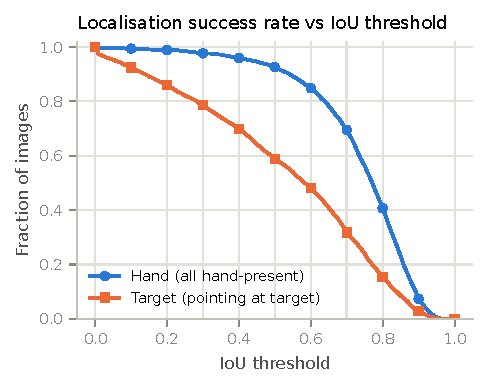
\includegraphics[width=0.48\linewidth]{figures/results/iou_success_rate}\hfill
  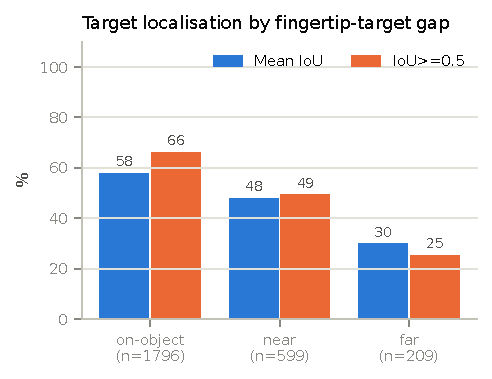
\includegraphics[width=0.48\linewidth]{figures/results/target_iou_by_gap}
  \caption{Left: share of test images whose hand or target box reaches each IoU threshold. Right: target mIoU and P@0.5 for touched, near and far targets.}
  \Description{Left: two curves of success rate against IoU threshold; the hand curve stays above 0.9 up to IoU 0.5 and falls after 0.7, while the target curve falls steadily, reaching 0.59 at IoU 0.5 and 0.32 at 0.7. Right: bars of mean target IoU and IoU above 0.5: 58 and 66 percent for touched targets, 48 and 49 for near targets, 30 and 25 for far targets.}
  \label{fig:curves}
\end{figure}

\paragraph{Hand presence.} The hand gate separates no-hand from pointing frames with 98.6\% accuracy (95\% CI 98.1--98.9) and AUROC 0.998. It misses 15 of 2,604 hands (0.6\%) and raises false alarms on 28 of 425 no-hand frames (6.6\%). Choosing the threshold on validation so that no hand is missed (0.22) removes the misses but raises false alarms to 117 (27.5\%), so we keep 0.5.

\paragraph{Where the errors come from.}
\begin{itemize}
\item \emph{Hand and fingertip are not the bottleneck.} The hand box and fingertip are equally good for all distances (hand P@0.5 of 92--94\%; about 4\,px fingertip error, 2.5\% of the image side).
\item \emph{The target falls off with distance.} Target P@0.5 drops from 66.0\% for touched targets to 49.2\% near and 25.4\% far (mIoU from 57.9 to 47.8 and 29.8).
\item \emph{The direction is coarse.} Its median error is 18.6$^\circ$, and only 36.8\% of far targets have an error below 15$^\circ$. At a median fingertip--target distance of 0.32 image widths, 15$^\circ$ already moves the ray by about 0.08 image widths, the size of a small object. The error is largest for touched targets (36$^\circ$), where the direction to the target centre is ill-defined and matters least.
\item \emph{Size is regressed towards the mean.} The predicted target centre lies inside the labelled box in 84.8\% of images. Giving the model the true size with its own centre would raise P@0.5 to 70.4\%; giving it the true centre with its own size would raise it to 72.3\%. Errors in position and in extent therefore contribute about equally. Small targets (under 3\% of the image) are predicted about 1.9 times too large, and reach a P@0.5 of only 36.9\%.
\end{itemize}

\subsection{Ablations}\label{sec:ablations}

We retrain the model without one component at a time, with the seed and settings of the main run:
\begin{itemize}
\item \textbf{A1} no distractor pasting and no ownership weighting;
\item \textbf{A2} no geometric consistency terms ($\mathcal{L}_{\mathrm{ray}}$ and the hand-axis term);
\item \textbf{A3} no ray conditioning of the target head (no $G^t$; 13,105 fewer parameters).
\end{itemize}
\tbd{A4 (recommended now that efficiency is the main claim): no instance-anchored chain, so the heads read the globally pooled vector (\texttt{--no\_anchor\_chain}). This is the same-size plain baseline; it shows whether the design, and not just the small backbone, explains the accuracy.}
Each ablation was trained once. Instead of seed variation, we report a paired bootstrap over test images: we resample the 2,604 images and recompute the difference between the full model and the ablation on the same images, which yields a 95\% confidence interval for each difference.

\begin{table}[t]
  \caption{Ablations (one seed each). Differences from the full model with 95\% paired-bootstrap intervals; intervals that exclude 0 are in bold. Ownership: ownership accuracy on the synthetic multi-hand test.}
  \label{tab:ablation}
  \footnotesize
  \setlength{\tabcolsep}{4pt}
  \begin{tabular}{lrrrrrr}
    \toprule
    Variant & Target mIoU & P@0.5 & Far P@0.5 & Hand mIoU & Tip (px) & Ownership \\
    \midrule
    Full model (seed 42) & 53.3 & 58.9 & 25.4 & 73.7 & 3.89 & 99.7 \\
    A1 no distractors / ownership weight & \xx & \xx & \xx & \xx & \xx & \xx \\
    A2 no geometric consistency terms & \xx & \xx & \xx & \xx & \xx & \xx \\
    A3 no ray conditioning & \xx & \xx & \xx & \xx & \xx & \xx \\
    \bottomrule
  \end{tabular}
\end{table}

\paragraph{Results.} \tbd{Write one claim per row, only as strong as its interval:}
\begin{itemize}
\item \tbd{A3 tests contribution C1. Far targets reach only 25.4\% with the ray conditioning; if A3 is not significantly lower, the ray prior does not help and C1 must be weakened in the abstract and introduction.}
\item \tbd{A2 tests whether the two consistency terms help, mostly on far targets.}
\item \tbd{A1 should mainly affect ownership; report any cost on clean-image accuracy. See the caveat in Section~\ref{sec:own}.}
\end{itemize}
The loss weights were not searched (Appendix~\ref{app:weights}): A2 covers the two non-standard terms, and the remaining eleven are standard box, keypoint, heatmap and focal losses.

\subsection{Following the Wearer's Hand}\label{sec:own}

\paragraph{Synthetic distractors.} With one or two pasted hands in each test image, the model's hand still lies nearer the wearer's hand than any pasted hand in 99.7\% of hand images (Table~\ref{tab:own}), and other metrics barely change. This is weaker evidence than it looks:
\begin{itemize}
\item The pasted hands follow the training distribution.
\item The ownership metric is easy under that distribution. In the first training epoch, when the hand IoU was only 0.38, ownership accuracy on training batches was already 93\%, because pasted hands sit in the upper part of the frame and the wearer's hand in the lower part.
\end{itemize}
The more informative number is that pasted hands rarely turn a no-hand frame into a hand frame: 91.8\% of no-hand frames stay \emph{no hand}, against 93.4\% without pasted hands. Whether the training recipe is needed at all is answered by A1, and robustness to real bystanders by the real-frame check below.

\paragraph{Real frames.} \tbd{Fill in when T5 is done:}
\begin{itemize}
\item We recorded \tbd{N} clips with the glasses in which another person's hand is visible, sometimes pointing, with \tbd{consent procedure}, and sampled \tbd{100--150} frames.
\item Two annotators independently labelled the predicted hand in each frame as the wearer's, another person's, or missed.
\item We report ownership accuracy with a Wilson interval and inter-annotator agreement (Cohen's $\kappa$).
\end{itemize}
Figure~\ref{fig:own-real} shows examples.

\begin{table}[t]
  \caption{Ownership on test images with one or two pasted hands (synthetic), and on real frames with other people's hands (T5). All values in \%. \emph{On other hand}: predicted hand centre inside a pasted hand. \emph{No hand kept}: no-hand images still classed as no hand.}
  \label{tab:own}
  \footnotesize
  \begin{tabular}{lrrrr}
    \toprule
    & Ownership accuracy & On other hand & No hand kept & Target P@0.5 \\
    \midrule
    Full model, clean test images & -- & -- & 93.4 & 58.9 \\
    Full model, pasted hands & 99.7 [99.4, 99.9] & 0.2 & 91.8 & 60.1 \\
    A1, pasted hands & \xx & \xx & \xx & \xx \\
    \midrule
    Full model, real frames (\tbd{N}) & \xx\ [\xx, \xx] & \xx & -- & -- \\
    \bottomrule
  \end{tabular}
\end{table}

\begin{figure}[t]
  \centering
  \phfig{\linewidth}{3.2cm}{Six real frames from the glasses with another person's hand in view: predicted wearer's hand, fingertip, ray and target (T5). Include at least one failure.}
  \caption{Real frames with other people's hands. \tbd{Insert after T5.}}
  \Description{To be inserted: six photos from the glasses showing SpatialNet's outputs while another person's hand is visible.}
  \label{fig:own-real}
\end{figure}

\subsection{On-Device Performance}\label{sec:ondevice}

Table~\ref{tab:device} reports cost on the evaluation machine and on the glasses.

\begin{table}[t]
  \caption{Inference cost at batch size 1 and $160\times160$ input. Server numbers use PyTorch eager mode on the 4-core Kaggle virtual machine used for evaluation and are given for reference only; at this model size, they are dominated by framework overhead.}
  \label{tab:device}
  \footnotesize
  \begin{tabular}{llrr}
    \toprule
    Platform and measure & Runtime / precision & Median & p90 \\
    \midrule
    Server CPU, 1 thread & PyTorch FP32 & 25.7\,ms & 28.0\,ms \\
    Server CPU, 4 threads & PyTorch FP32 & 25.8\,ms & 27.0\,ms \\
    Server GPU, NVIDIA Tesla T4 & PyTorch FP32 & 15.9\,ms & 16.3\,ms \\
    \midrule
    Glasses, model only & \tbd{runtime, unit, precision} & \xx\,ms & \xx\,ms \\
    Glasses, camera frame to result & \tbd{same} & \xx\,ms & \xx\,ms \\
    Glasses, sustained throughput (60\,s) & & \multicolumn{2}{r}{\xx\ frames/s} \\
    Glasses, peak memory / battery per 10\,min & & \multicolumn{2}{r}{\xx\,MB / \xx\%} \\
    Glasses vs.\ PyTorch, 100 test images & & \multicolumn{2}{r}{\xx\% same scene; box IoU \xx} \\
    \bottomrule
  \end{tabular}
\end{table}

\paragraph{Results.} Running the FP16 weights in half precision gives the same target IoU as FP32 on 320 validation images (0.510 in both), so halving the model size costs no accuracy. \tbd{T2: model latency against the camera's frame interval, end-to-end latency against a 100--200\,ms interactive budget, and the cost gap to the GPU-based models of Table~\ref{tab:main} (VistaRef: 22.9 images/s on a GPU). If capture or conversion dominates the end-to-end time rather than the model, say so.}

\subsection{Qualitative Results and Failure Analysis}\label{sec:qual}

Figure~\ref{fig:qual} shows typical successes and failures. We sorted the 558 test images with target IoU $<$ 0.3 (21.4\%) by rule:
\begin{itemize}
\item \emph{Right object, wrong extent} (36\%): the predicted centre lies inside the labelled box. These are mostly touched targets (137 of 199), for example part of a bed instead of the whole bed.
\item \emph{Wrong direction} (33\%): direction error over 45$^\circ$.
\item \emph{Wrong object despite a reasonable direction} (31\%): mostly near and far targets (130 of 171), typically a similar object next to the labelled one along the ray.
\item \emph{Hand missed} (1\%).
\end{itemize}
Some labelled targets are ambiguous: in the ``wrong direction'' example, the finger touches the bowl but the label is an apple above it. \tbd{Inspect a random sample of 50 failures and report the share with a questionable label.}

\begin{figure}[t]
  \centering
  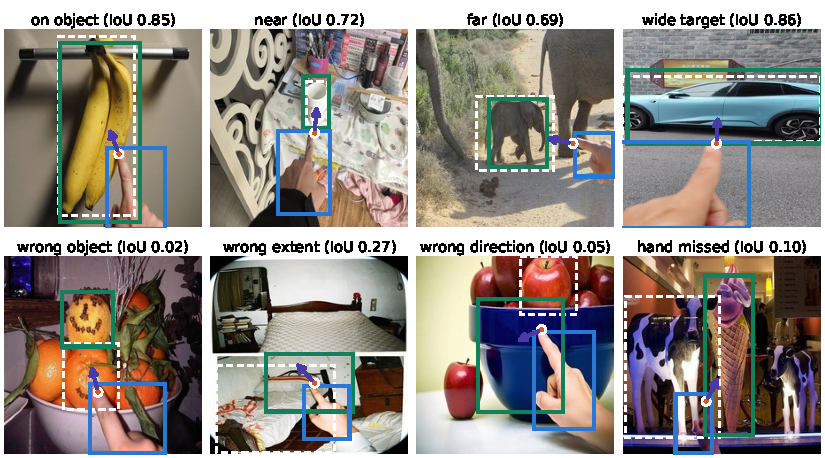
\includegraphics[width=\linewidth]{figures/qualitative}
  \caption{Successes (top) and failures (bottom) on EgoPoint test images: predicted hand (blue), fingertip and direction, and target (green); labelled target dashed. Bottom row, one example per failure type of Section~\ref{sec:qual}.}
  \Description{Eight egocentric images. Top row: correct target boxes for bananas touched by the finger, a cup near the finger, a young elephant far from the finger, and a car. Bottom row: a box on the wrong orange in a bowl of oranges, a box on part of a bed instead of the labelled bed, a box on a bowl while the label is an apple above it, and a frame where the hand gate missed the hand.}
  \label{fig:qual}
\end{figure}
